\chapter{Fundamentos Teóricos y Técnológicos}
\label{chap:ft}
\lettrine{E}{n} este capítulo se repasan los principios básicos sobre los que se establece este trabajo.
\section{Tomografía Computerizada}

Una \acrfull{tc}, también conocida como escáner, es una técnica de
diagnóstico médico que utiliza rayos X, detectores y un ordenador para
obtener imágenes detalladas de estructuras internas del cuerpo. La
\acrshort{tc} combina una serie de imágenes radiográficas en secciones
transversales para crear imágenes en 2D y 3D del área estudiada.

Durante una \acrshort{tc}, el paciente se coloca en una mesa que se
desliza dentro de un dispositivo circular llamado tomógrafo. Un
tomógrafo es, en esencia, una máquina de rayos X en la cual se ha
sustituido la placa por una serie de
detectores~\cite{muniz2006introduccion}. La fuente de rayos X y los
detectores efectúan un movimiento circular y avanzan lentamente hasta
cubrir el área deseada, como se puede ver en
\figurename~\ref{fig:tac}. Los detectores capturan la radiación
después de que ha atravesado el cuerpo. La información recopilada se
envía a un ordenador que procesa los datos y los convierte en imágenes
transversales o en secciones longitudinales del área de interés.

\begin{figure}%
    \centering
    \subfloat[\centering Orientación del tubo de rayos X respecto al eje corporal.]{{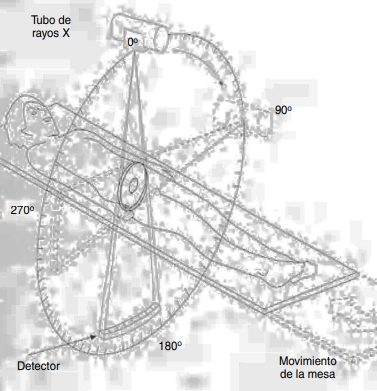
\includegraphics[width=5cm]{imaxes/tac.png} }}%
    \qquad
    \subfloat[\centering Tomografía axial computerizada convencional.]{{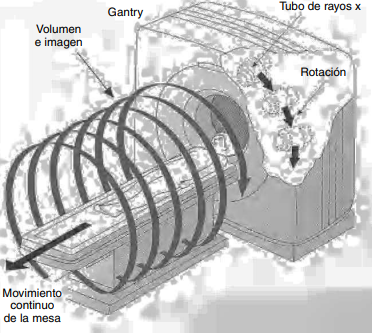
\includegraphics[width=5cm]{imaxes/tacm.png} }}%
    \caption{Representación del funcionamiento de un \acrshort{tc}}%
    \label{fig:tac}%
\end{figure}

La tomografía computarizada proporciona imágenes detalladas de tejidos
blandos, huesos y órganos internos, lo que permite a los médicos
diagnosticar y evaluar una amplia variedad de condiciones y
enfermedades. Se utiliza comúnmente en el diagnóstico y seguimiento de
enfermedades como cáncer, lesiones traumáticas, enfermedades
cardiovasculares, trastornos pulmonares, afecciones cerebrales y
abdominales, entre otros.



\paragraph{Teorema de Radon.}
Propuesto por el matemático austríaco Johann Radon en 1917, el Teorema de Radon es un resultado fundamental en la teoría de la tomografía computerizada. Este teorema establece que es posible reconstruir una función bidimensional a partir de sus proyecciones a lo largo de diferentes ángulos. En el contexto de la tomografía computerizada, las proyecciones se obtienen mediante la medición de la atenuación de la radiación a medida que atraviesa el objeto en estudio.
%En una TC, se obtienen múltiples proyecciones de rayos X mientras el tubo de rayos X y los detectores giran alrededor del paciente. Estas proyecciones se toman desde diferentes ángulos y se utilizan para capturar información sobre cómo los tejidos dentro del cuerpo absorben los rayos X.
Una vez que se han recopilado todas las proyecciones, se utiliza un algoritmo de reconstrucción para combinarlas y generar una imagen transversal detallada del área estudiada. La base matemática de ese proceso de reconstrucción de imágenes en la tomografía computerizada la proporciona el teorema de Radon y ha llevado al desarrollo de diversos algoritmos de reconstrucción.


\paragraph{Algoritmos de reconstrucción de imágenes.}
Los algoritmos de reconstrucción de imágenes son métodos computacionales utilizados para reconstruir imágenes bidimensionales o tridimensionales a partir de proyecciones adquiridas en la tomografía computerizada. Estos algoritmos se basan en el Teorema de Radon y pueden clasificarse en dos categorías principales: métodos analíticos \cite{kontaxakis2002reconstruccion} y métodos iterativos \cite{Willemink2013}.

1. Métodos analíticos: Estos algoritmos, como la retroproyección filtrada (FBP, por sus siglas en inglés), procesan las proyecciones de manera directa para obtener la imagen reconstruida. La FBP es el algoritmo más utilizado en la práctica clínica debido a su rapidez y eficiencia.

2. Métodos iterativos: Estos algoritmos, como el de máxima verosimilitud de la expectativa-maximización (MLEM) y el de mínimos cuadrados conjugados (CGLS), utilizan un enfoque iterativo para mejorar la calidad de la imagen reconstruida. Aunque estos métodos suelen ser más lentos que los analíticos, pueden proporcionar imágenes de mayor calidad y son especialmente útiles en aplicaciones donde la cantidad de datos de proyección es limitada o ruidosa.



\section{Impresión 3D}

La impresión 3D es una tecnología de fabricación aditiva que permite crear objetos tridimensionales a partir de un modelo digital. Esta tecnología ha revolucionado la forma en que se fabrican piezas y productos, ya que permite la creación de objetos complejos con geometrías que serían difíciles o imposibles de lograr con métodos de fabricación tradicionales. La impresión 3D se utiliza en una amplia variedad de aplicaciones, desde la fabricación de piezas de repuesto hasta la creación de prótesis médicas personalizadas.

\paragraph{Fabricación aditiva.}
La impresión 3D es un ejemplo de fabricación aditiva, que se refiere a manipulación y deposito de un material a escala micrométrica de forma muy precisa para construir un sólido. La fabricación aditiva es una alternativa a los métodos de fabricación tradicionales, como el fresado y el torneado, que implican la eliminación de material de una pieza bruta \cite{zahera2012fabricacion}.

Esta técnica de fabricación presenta una serie de ventajas. La complejidad de la geometría de la figura no encarece la fabricación de la misma (a expensas de la necesidad de material como soporte de la geometría principal) sino que permite generar piezas con geometrías previamente inviables, o con un alto coste.
Otra de las ventajas es la posibilidad de generar prototipos de piezas cuyas versiones finales presentan un alto coste, por un precio muy reducido, y una alta fidelidad acelerando así el proceso iterativo del diseño.

\paragraph{Modelado.}
El proceso de impresión 3D comienza con el modelado de la pieza o producto que se desea imprimir. Este modelo puede crearse utilizando software \acrfull{cad} o mediante la digitalización de un objeto existente utilizando un escáner 3D. En nuestro caso, el modelo tridimensional se obtiene de la reconstrucción 3D a partir de una \acrshort{tc}.

\paragraph{\emph{Slicing} (rebanado)}

En impresión 3D, el proceso de slicing (o rebanado, en español) se refiere a la preparación del modelo tridimensional, típicamente en formato STL, para su impresión en capas sucesivas. Es un paso crucial que convierte el modelo en una serie de capas planas y delgadas que la impresora 3D puede imprimir una por una.
El \emph{slicer} permite además realizar ajustes en el modelo 3D, con el fin de obtener el resultado deseado, generando como resultado una serie de instrucciones precisas que la impresora entiende para elaborar capa a capa el volumen.

\paragraph{GCODE.} Las instrucciones que se generan a partir del proceso de \emph{slicing} son provistas en forma de GCODE. El GCODE es el lenguaje utilizado para describir paso a paso que movimientos y acciones debe tomar la impresora en cada momento. Este lenguaje tiene distintas implementaciones dependiendo del fabricante del equipamiento, ya que se trata de un lenguaje utilizado en múltiples aplicaciones de control numérico.

\section{Realidad Extendida}

\acrfull{xr} es un término general que engloba todo el espectro de tecnologías inmersivas, incluyendo \acrfull{vr}, \acrfull{ar} y \acrfull{mr}. \acrshort{xr} se refiere a la fusión de los mundos físico y digital, creando un entorno inmersivo que puede incluir objetos virtuales, información digital y elementos del mundo real.

En 1994, \citeauthor{Milgram1994ATO}~\cite{Milgram1994ATO} acuñan el término de \emph{virtuality continuum}, que representa una escala que comprende desde la realidad física pura hasta la realidad virtual total, abarcando diferentes niveles de inmersión e interacción. Este \emph{continuum} describe así la gama completa de experiencias, desde la realidad física no modificada hasta entornos completamente virtuales, como se muestra en la \figurename~\ref{fig:vc}:
\begin{itemize}
    \item Entorno Real: consiste únicamente en objetos reales (extremo izquierdo de la figura).
    \item Realidad Aumentada: mundo real aumentado o compuesto por elementos digitales.
    \item Virtualidad Aumentada: mundo digital aumentado por objetos reales o fisicos.
    \item Entorno Virtual: entorno puramente virtual (extremo derecho de la figura).
\end{itemize}

\begin{figure}
  \centering
  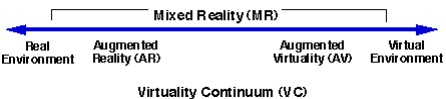
\includegraphics[width=0.6\textwidth]{imaxes/virtuality_continuum.png}
  \caption{Representacion simplificada del concepto de \emph{virtuality continuum}.}
  \label{fig:vc}
\end{figure}

\paragraph{Realidad aumentada.}
Posteriormente \citeauthor{Azuma1997}~\cite{Azuma1997} definía la \acrlong{ar} como una variación de la \acrlong{vr}, en la cual el usuario es capaz de ver el mundo real, con objetos virtuales superpuestos, o compuestos por el mundo real. La posibilidad de crear objetos y prototipos de forma rápida, sobre los cuales poder iterar y componer imágenes virtuales, demuestra el potencial de estas tecnologías inmersivas trabajando a la par. En la actualidad sus principales aplicaciones se encuentran, además de en juegos y entretenimiento, en educación, medicina, arquitecture, ingeniería e interpretación del patrimonio.

%La realidad aumentada es una tecnología que combina elementos virtuales con el mundo real, permitiendo a los usuarios interactuar con objetos y escenarios virtuales en tiempo real.

\section{Visión Artificial}

Se denomina visión artificial al campo que incluye los métodos necesarios para adquirir, procesar, analizar y comprender las imágenes del mundo real con el fin de producir información procesable por un ordenador. Esta fuertemente vinculado con la realidad aumentada, ya que es imprescindible para poder transmitir la información del medio al ordenador encargado de generar imágenes correspondientes. 
Entre los objetivos de la visión artificial se encuentra la capacidad de reconocer patrones dentro de una imagen o vídeo con el fin de poder extraer las características de los objetos dentro de dicho medio y  procesarlas. 
Otro objetivo es la reconstrucción 3D a partir de imágenes, que pretende generar volúmenes 3D desde las imágenes obtenidas, esto es especialmente importante en la realidad aumentada por que permite una mayor percepción de la profundidad sobre el medio generado por ordenador.